% Chapter 3

\chapter{Improvements on the Existing System} % Main chapter title

\label{Chapter3} % For referencing the chapter elsewhere, use \ref{Chapter1} 

%----------------------------------------------------------------------------------------

\section{Developing Modules for Nukeboard}

\subsection{What is a Module?}

A \textbf{\textit{module}} is a part of a software that performs a particular task. Modules consist of routines which talk together to perform the goal in which the module is built for. A module can also be termed a feature for a software. Modules make the development of a software easy to understand and if there is a problem in the software, trouble-shooting is very possible and the solution to the problem is easy to find.

\subsection{Modules for Nukeboard.co}

Nukeboard.co has a total of 5 modules and they are listed below as follows;
- Job Seeker Module. \\
- Employer Module. \\
- Blog Module. \\
- Training Module. \\
- Sponsored Jobs Module. \\

\begin{figure}[h]
\centering
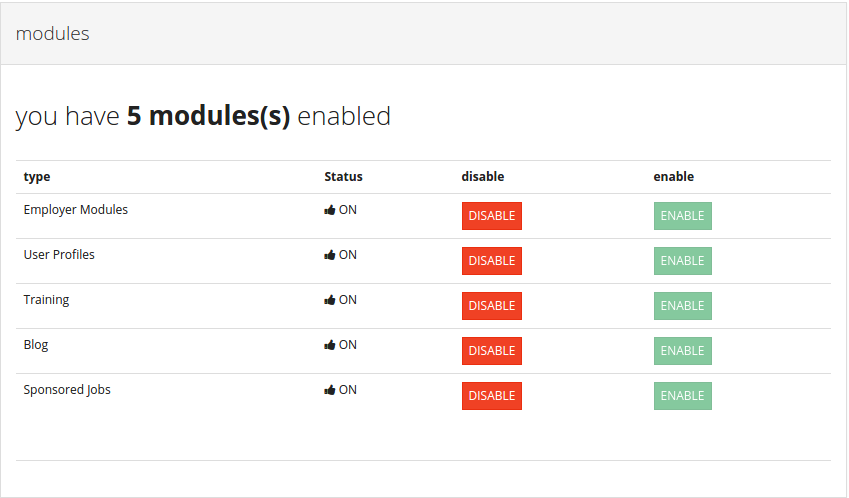
\includegraphics[width=13cm,scale=1.5]{Figures/Modules}
\decoRule
\caption[Nukeboard Modules]{Modules in nukeboard.co}
\label{fig:Modules}
\end{figure}

The above listed modules where all developed during my Internship program by a team of engineering interns in which I was included. I will briefly describe the meaning or goal of the modules and further more focus on the one is which I worked on during my internship period. Also, it should be noted that all the work done during my internship period where translateable from English to French and vise versa. But if there is something specific about the translation, I will do a quick mention.

\subsubsection{Job Seeker Module}

Job Seeker module is used by "job seekers"(applicants seeking for jobs) to apply for available jobs on nukeboard.co and with the Job seeker module, the application process for a job is really easy since most of the work is already done by the programmers and job seekers just need a few more steps to complete the process. When a job seeker has an account on a job board(if the module is activated on that job board), applications to jobs is really simple because he/she(applicant) just needs to click "Apply" and his application is sent to the job owner without filling forms because this is done when the job seeker is creating his/her profile. But if a job seeker who hasn't a job seeker account wants to apply for a job, he/she will need to fill a form(anonymously) for the application process. \\

Also, administrators of a job board where the "Job Seeker Module" is activated also do their task easily since applications are tracked and rendered to them in the backend of the job seeker module is a nicer and more presentable manner so that they can just read through the application an continue with the recruitement process easily.

\subsubsection{Employer Module}

This module handles the management of employers under a particular job board. A company can have a job board and wants the employer module to be activated. This enables employers to create accounts on the company's job board and also make job offers available to the public. Meanwhile job board owner can post jobs to thier job board, employers under that job board can also post jobs making the availability of jobs under that job board richer and more for the public. Job board owners can post jobs as employers if the employer has a job but not available to post the job at the moment. \\

Also, job board owners can manage the employers on their job board, suspend them in case of any suspicious action, view the jobs posted by the employers etc \ldots All these is done from the Employer module backend

\subsubsection{Blog Module}

Blog module enables owners of job board(if activated) to blog about jobs offers, opportunities and more\ldots This module works exactly how Blogs work, applicants, anonymous users, registered users can blog about anything but this module is highly controlled by the admins of the job board because users can blog about irrelevant and indecent issues and if this is done, these blogs will be removed from the job board by the admins. Like other modules, this module has its own backend for managing blogs. \\ 

When a blog is posted, users can comment and say something about the blog, this is done so by the means of a Facebook Comment plugin which has been integrated in the blog module. And when this is done(commenting on a blog) you can access this blog from your Facebook page since its a Facebook plugin.

\subsubsection{Training Module}

Its a very important module that also solves a big problem in the society concerning job offers. If a particular job needs training before the job being done or there is a training offer that needs to be carried out in order for job seekers to acquire the necessary skills needed to perform or do a job, this offers are posted using the Training module. This is done for specificity not to mix training offers with job offers. Training module has a backend for the management of training, update of training, delete, and more\ldots \\

Important parameters of a training offer can be the duration of the training, maximum number of students or applicants, price tag per duration and per student within the particular training duration, etc...

\subsubsection{Sponsored Jobs Module}

Sponsored Jobs is a module that increases the priority of a normal job offer, if owners of a job board or employers under a job board mark jobs as sponsored(if this module is activated for that job board), these jobs are posted at the job of the Jobs page and it makes the priority of the job high. This is a call for attention to job seekers making sure that they see the sponsored jobs first and apply for them. Jobs under this module are more lucrative. \\ 

This module also has a backend in which it is used to manage sponsored jobs posted on the job board, making it easy to track which jobs are sponsored and which ones are not.

\textbf{Note:} Any activity happening a job board is not visible to another job board. This condition is carefully handled in order not to mix things up and lose tracking of activities across various job boards. Its a critical problem that is solved at the level of the Database design. Example; If job board A is carrying out activies, its only shown in job board A and if another job board B is carrying its own activites, its not shown in A. So if a module(Employer module) is activated in job board A, it does not show in B etc...

\section{Tasks I completed during my Internship period}

First of all, since I was working on developing modules, there is a contraint about these modules. It must be activated by the job board owner or job board admin before its visible on the job board.

\subsection{Implemenation of EmployerSessionController.php Class}

I wrote a class that was responsible for managing session activities in the employer module. The class was named EmployerSessionController { }  which extended the Laravel's BaseController { } class and its was given a file named EmployerSessionController.php. A template code can be found below as regards the declaration of the class; \\

\begin{lstlisting}

<?php

class EmployerSessionController extends BaseController
{

}

\end{lstlisting}

This class handled functionalities like; employer login, employer logout, employer recover password, employer create account(register). All these was done by routines that were called using the routes.php file when an employer wants to perform any of these actions. After working on these controller/class, the pages linked to it for example when a employer logs in, he/she has to be redirected to the employer backend home page if authentication was successful. So all the pages that are linked to this controller had to be translatable from English to French and vise versa. Note that, the translation we(development team for nukeboard) did was proof read by a professional translator hired by the owner of the project, if any mistakes, it will corrected to make sure that the French version of the software was perfect.

\subsection{Implemenation of Permission in nukeboard core}

Job board owners needed permission to control Employers and Job seeker accounts if in the case of any suspicious actions for example Scam. The admin of the job board needed this permission so that if a fraudulent action is detected, the user involed will be suspended from accessing the account till the problem is rectified and this part of my work was done in the nukeboard.co core itself. It was not a module in nukeboard.co. \\

The various permissions that were available to the job board admin was; 
- Approve. \\
- Suspend. \\

With this permissions available, I had to create an interface in which the job admin can view all users(both employer and job seeker) so that it will be easy to perform this operations.

\subsection{Built Registration Wizard for Employer and Job Seeker Module}

Both the Employer module and the Job seeker module needed wizards registration wizards to make sure that all the information about the users of these modules are completely collected. This was a serious improvement to the software since after this task was completed we never bordered to think about us not having the necessary information about the users of the module since we knew that all was collected following the wizard. Below is a description of what I implemented for each module.

\subsubsection{Registration Wizard for Employer Module}

After an employer finishes creating his/her account, he/she is registered to the nukeboard.co database with account status "pending" and asked to login to update his/her account. If the employer logs in, a wizard will start automatically enabling and guiding at each step telling the user to input the required information at each step. The first welcome window that the employer sees is: 

\begin{figure}[h]
\centering
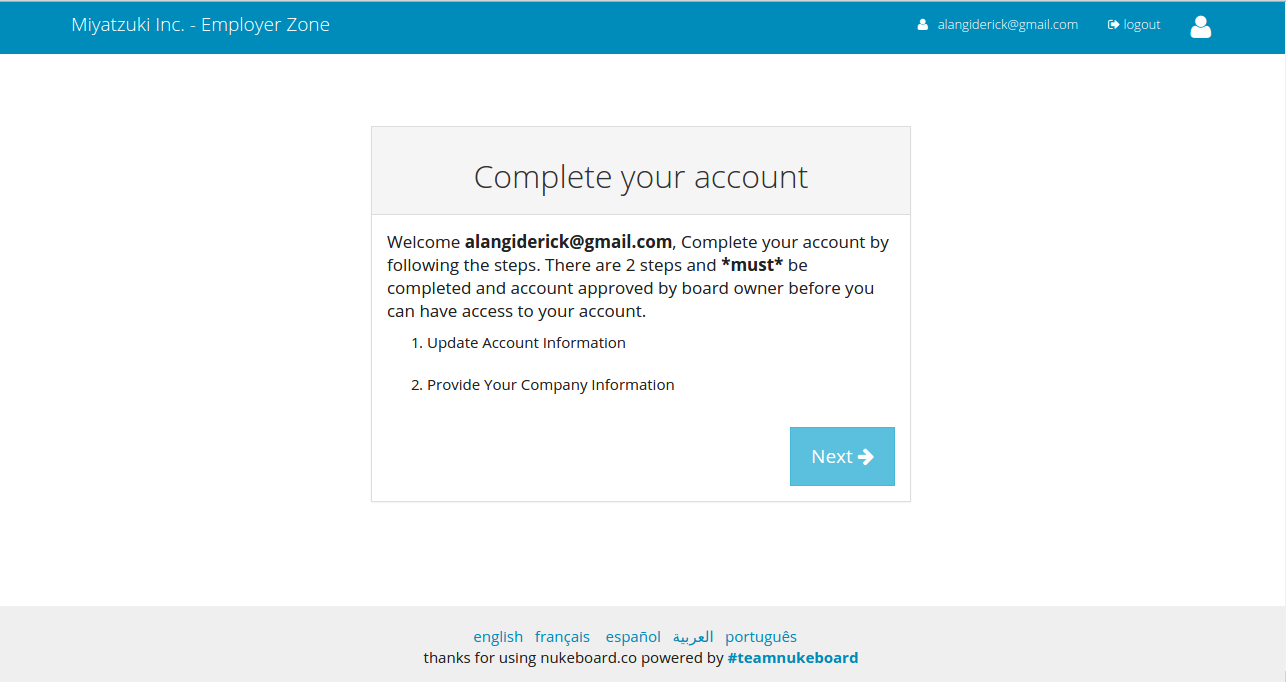
\includegraphics[width=13cm,scale=1.5]{Figures/EmployerWizard}
\decoRule
\caption[Employer Wizard]{Registration Wizard for the employer module Welcome page}
\label{fig:EmployerWizard}
\end{figure}

Two sets of information are collected from the employer and saved in the nukebaord.co database which are the;\\
- Account Information and \\
- Company Information. \\

\textbf{Account Information} is the information partaining to the account created by the employer like; First Name, Last Name, Telephone Number etc\ldots  \textbf{Company Information} requires the employer to provide the information about the company he/she is working with. Information about the company like; Logo, Company name, Company Website (if any) etc\ldots. When all these information is gotten by the wizard, the account creation is complete and a request is sent to the board owner to either approve or reject this employers account and if its approved, the employer can now have full access to his/her account and start posting job offers and managing the backend. \\

If in the process of submitting information entered at each step of the wizard and there is an error, the wizard redirects back to the previous step with the old data inputed so that the user will not need to enter the whole set of information again. After each step is successfully completed, the information is saved immediately in the database to prevent information and for the user start the process all over again in case of power outage or internet failure. Meaning that if any of these disasters happen, when the employer logs into his/her account, he/she will just continue with the process without starting all over.

\begin{figure}[h]
\centering
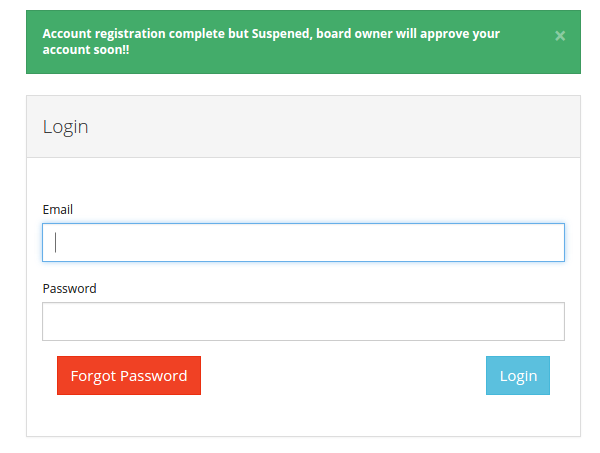
\includegraphics[width=13cm,height=7cm,keepaspectratio]{Figures/EmployerWizardComplete}
\decoRule
\caption[Employer Wizard Complete]{Completion of Employer Wizard}
\label{fig:EmployerWizardComplete}
\end{figure}

The entire employer wizard process is translateable meaning that it was both in English and French. This task was completed successfully and reviewed by the project lead and owner. It was a major improvement to the project and clients loved the purpose of it.


\subsubsection{Registration Wizard for Job Seeker Module}

When a job seeker creates an account under a particular job board, his/her information is added to the nukeboard database and when he/she tries logging into their accounts, a wizard starts up which is to collect their information to update their accounts and others. This time around, unlike the employer registration wizard, there is a slight diference with this one, after collecting the information partaining to the account as for employer account, the next step is to collect information about the first job of the job seeker. This set of information will tell the recruiters how much experience the job seeker has in his/her field of work.

\begin{figure}[h]
\centering
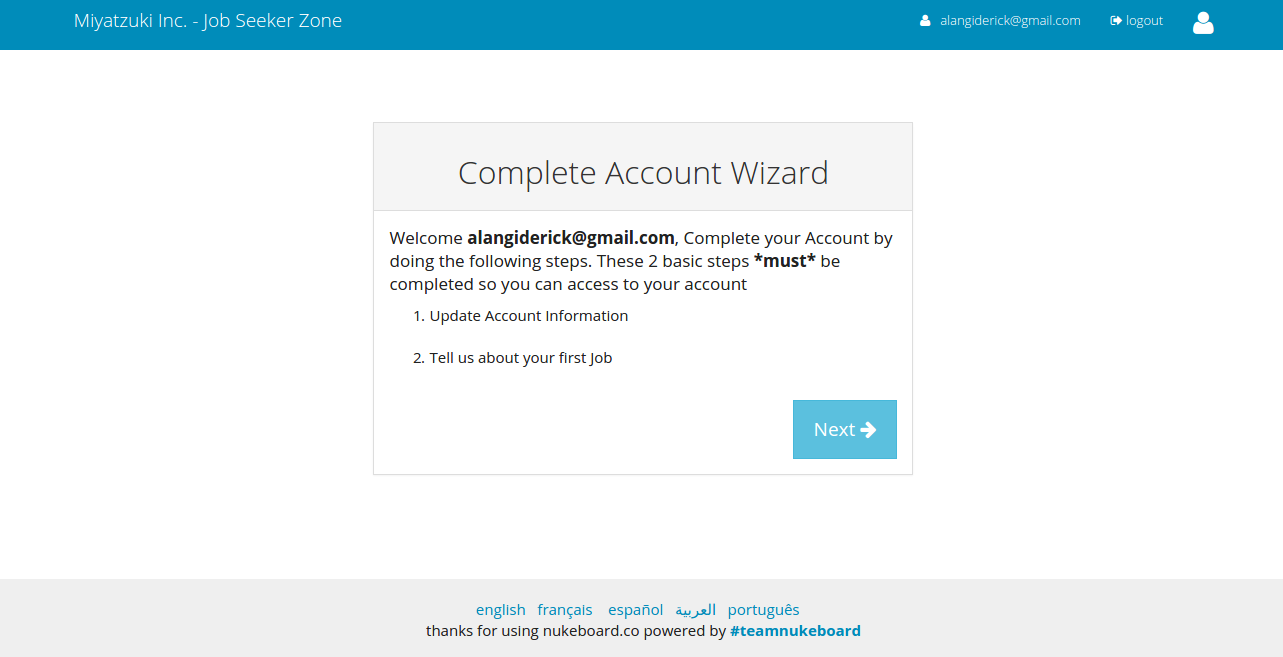
\includegraphics[width=13cm,scale=1.5]{Figures/JobSeekerWizard}
\decoRule
\caption[Job Seeker Wizard]{Wizard welcome page for Job seekers}
\label{fig:Modules}
\end{figure}

This wizard is very similar to the employer registration wizard in terms of information saving in the database after each step to prevent information loss in case of internet failure and power failure. Also redirection with old input to prevent users from inputing the same information again over and over. Informations like date of birth is collected in the account information of the job seeker to know his/her age so that if there is job with an age range, this will enable recruiters to filter applicants/job seekers based on age, experience and age range. This will be further explain ahead in the report.

In addition, by default when a job seeker creates an account he/she has access to it immediately so the he/she can start applying for job offers matching his/her required skill set.

\subsection{Changes and Migration of Employer and Job Seeker Themes}

Due to the too much similarity of them Employer and Job Seeker themes with the job site, there was a need to migrate this into two separate entities and change the theme completely so that the users of these sections of the software will have a feeling of difference and also privilledge that they are different from the normal users. When we met the system, admins theme for these modules where the same with the job site making them to feel as if they are still using the system as normal user. \\

This was a great improvement on the system since the change in the theme for admins separated them from the normal user mode to a different environment. They felt as if there were working on a different level of abstraction in the software making them feel superior and more confortable in their position as admins. Below is the current theme used by the admins of the various modules and this them match the theme used by the job board owner when he/she access the backend of the his/her job board.

\begin{figure}[h]
\centering
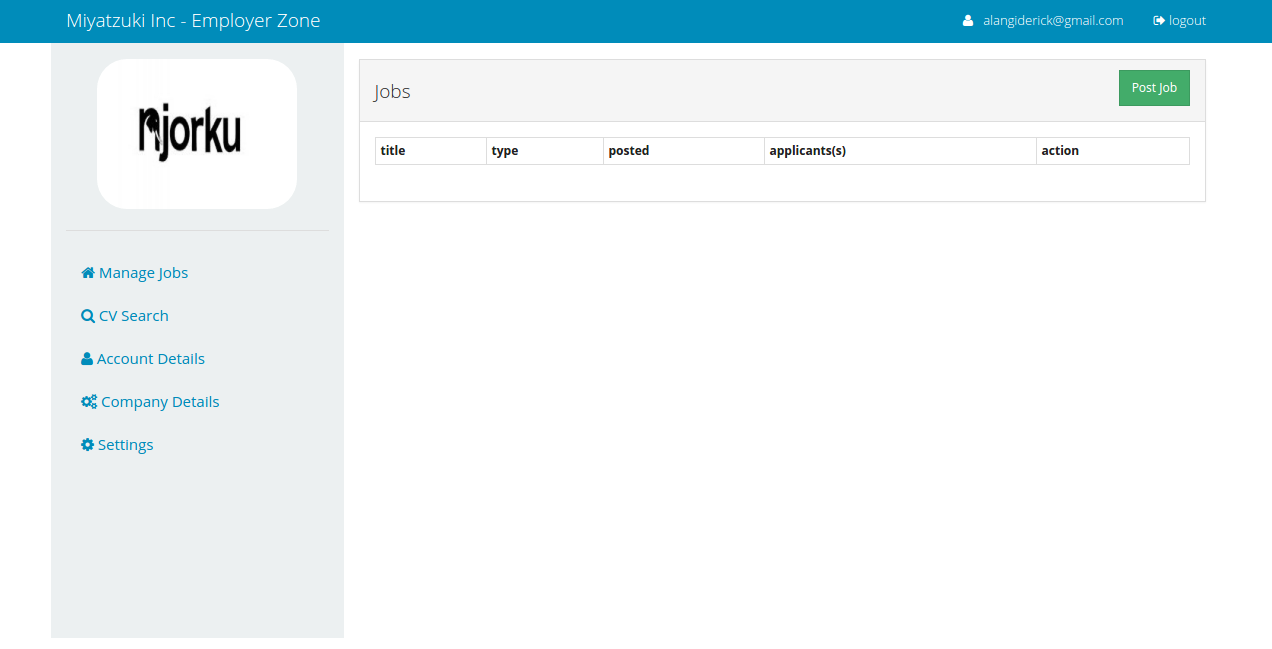
\includegraphics[width=13cm,scale=1.5]{Figures/ThemeEmployerModule}
\decoRule
\caption[Employer Module Theme]{Theme used by employer module and other modules in nukeboard.co}
\label{fig:Modules}
\end{figure} 

Like I earlier mentioned, this same theme is used by all the modules in nukeboard.co and also the backend for the job board owner uses the same theme.

\subsection{Implentation of CV Search on Nukeboard(nukeboard.co)}

CV's of job applicants where saved in nukeboards cloud server where they can later on be searched based on particular search criteria. These CV's are uploaded as .pdf, .doc, .docx files. Since the CV search functionality was available for both the Employers and the nukeboard.co core, it was necessary that employers and job board owner would search for CVs matching particular criteria to speed up their recruitement process. There are two kinds of CV search methods available;
- General CV search approach. \\
- Specific CV search approach. \\

When CVs collected by nukeboard.co is uploaded to the servers, a dump of the text in the CVs is collected using Apache Tika which parses these files and dumps the text in each CV into the database. This is to make sure that when keywords are searched in applicants CVs, it will be possible to find as text since there is not possibility to search in a .pdf document and more\ldots

\subsubsection{General CV Search Approach}

This is a search method in which all CV's matching a particular keyword are returned. Given a keyword like "engineering", searching through the index table of nukeboard will return all applicants CVs matching the keyword "engineering" or CVs that have the keyword "engineering". The applicants having these CVs are returned in a long paginated list which can be viewed by the recruiter. Below is a sample output search.

\begin{figure}[h]
\centering
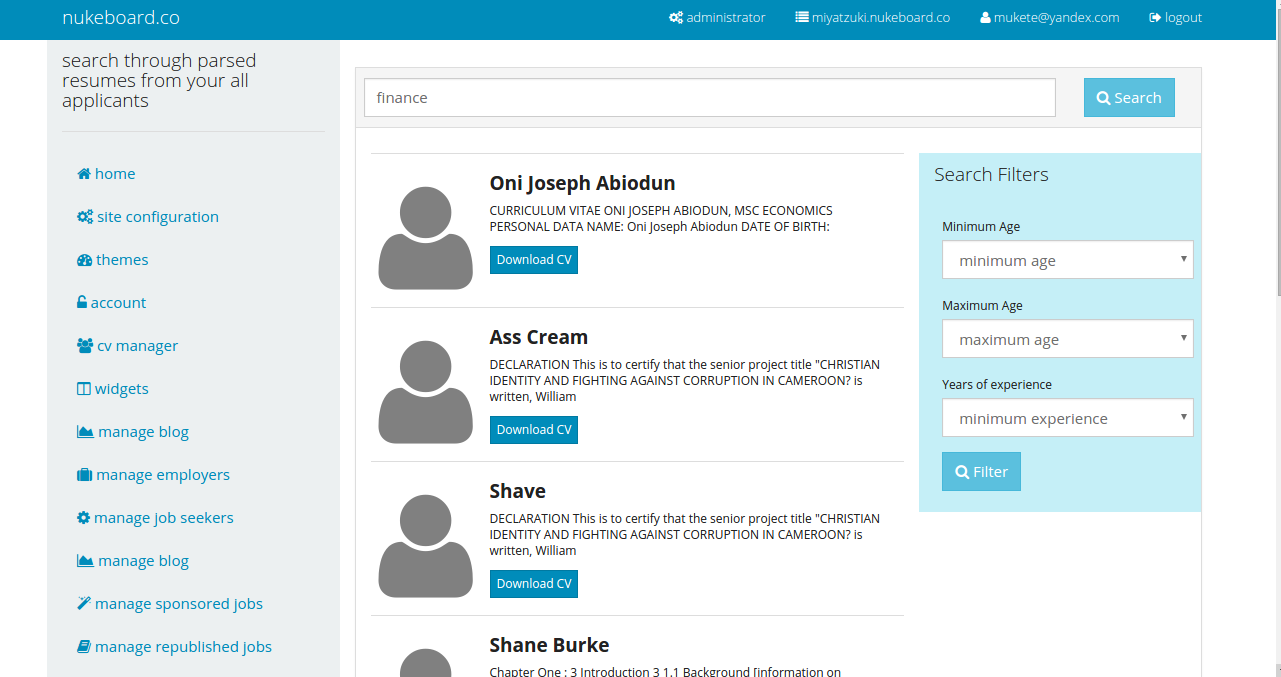
\includegraphics[width=13cm,scale=1.5]{Figures/cvGeneralSearch}
\decoRule
\caption[General CV Search Approach]{General CV Search, Keyword "finance"}
\label{fig:cvGeneralSearch}
\end{figure} 

The output of the General CV search is too vaque because a list of all CVs matching the keyword criteria will be rendered. Also, this search was already existing in nukeboard before I joined the development team so my own part of the work was to make the search specific so that recruiters can narrow down their search result making it easy for them to recruit job seekers.

\subsubsection{Specific CV Search Approach}

The specific CV search approach used the general CV search method including filters for narrowin down the search results. These filters where; age, age range and experience. Recruiters might want to quicken their search and also recruite job seekers in a particular age range with a particular level of experience, so a general search will not solve the problem since the recruiter will have to go all the CVs returned by the general search to pick out this applicants which is very stressful and adds more work to the users of the system. So I solved this problem so that recruiters can specify their search using filters to narrow down their search and pick out the required job seekers to employ. A sample output for this search can be as follows;

\begin{figure}[h]
\centering
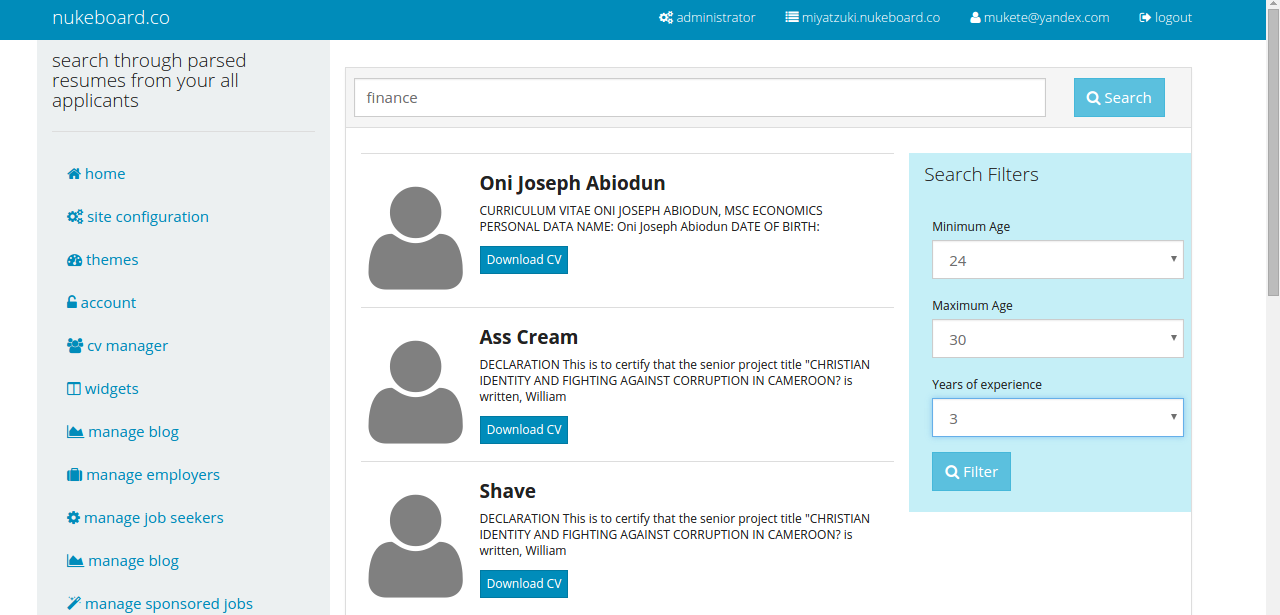
\includegraphics[width=13cm,scale=1.5]{Figures/SpecificCVSearch}
\decoRule
\caption[Specific CV Search Approach]{Specific CV Search, Keyword "finance" and filters}
\label{fig:SpecificCVSearch}
\end{figure} 

This search approach greatly solved the problem that the recruiters faced using the general search approach. In addition, the general search approach was a slower considering the time required to search and return all the CVs have to be searched but the specific CV search was faster since searching the CV was based on not only the keyword but on three different filters; minimum age, maximum age and years of expirience. So to wrap up, the more the filters, the faster the search but in future, we are to improve on the search speed using a different search algorithm not the filters. \\

In addition to the search results, presentability was a problem to the clients using the system so it was necessary to make the results look very presentable with a download button beside each applicant so that his/her CV can be directly downloa and his/her profile can be viewed by the recruiter. In the search results, applicants with profile pictures, their pictures where displayed and those without pictures, a default glyphincon-user was placed showing there is no picture.

\subsection{Implentation of Sponsored Jobs Module Front-end(FE)}

As I described the Sponsored jobs module above, I was required during my internship period to work on the front-end display of the sponsored job on all the themes available in nukeboard.co. My task was to get all jobs from the database and render them in a specified location(top of all jobs) in the nukeboard job board themes. A snapshot of sponsored jobs in the search green theme below

\begin{figure}[h]
\centering
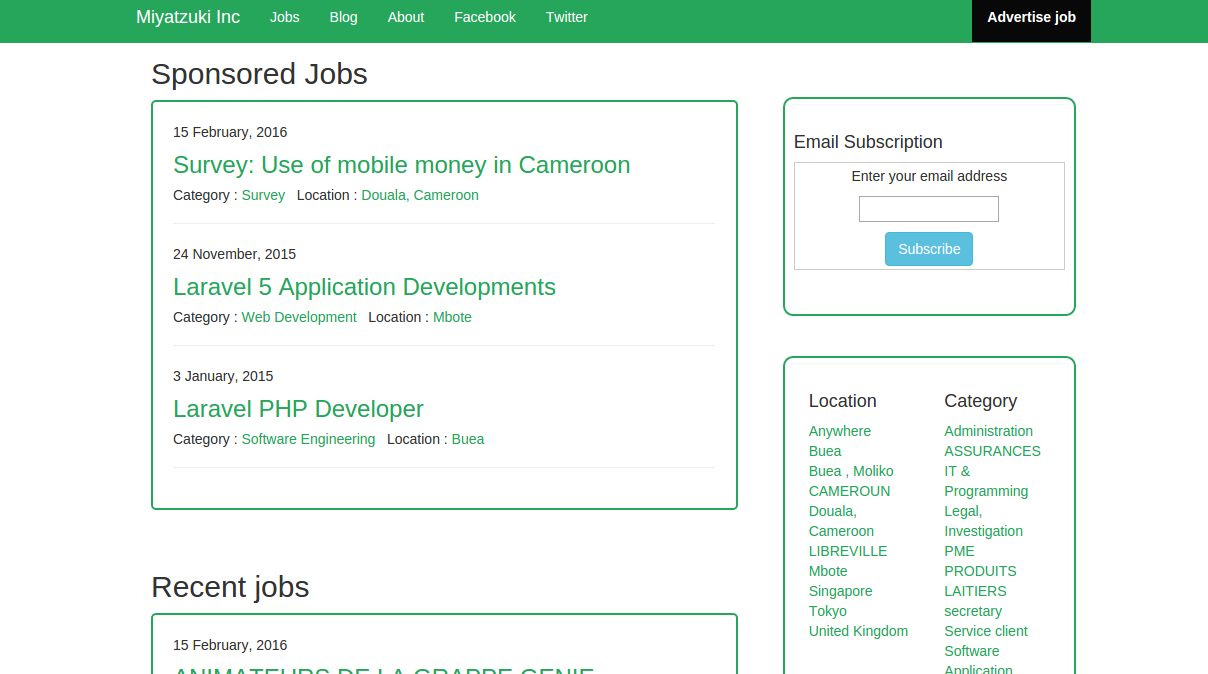
\includegraphics[width=13cm,scale=1.5]{Figures/SponsoredJobFE}
\decoRule
\caption[Sponsored Jobs Front-end]{Sponsored jobs, search green theme.}
\label{fig:SponsoredJobFE}
\end{figure} 

A field was added to the DB jobs table to check if a job is marked sponsored or not. My job was to go through this field and check if its marked sponsored and any corresponding field marked sponsored has a job ID attributed to it and I will just query all the jobs that are marked sponsored from the jobs table.

\subsection{HTML Email support for Nukeboard(nukeboard.co)}

When I join the project, nukeboard had email support and was already sending emails when needed but the emails where not presentable and did not look nice to the user/clients. There was a need to improve on the email structure and design for nukeboard. So the project owner decided that HTML emails should be implemented also known as styled emails. The task was assigned to me and I searched online for HTML email templates and i stumbled on one. I proposed it to the nukeboard team and it was agreed that i should use it. \\

I went ahead and replaced some of the plain-text email into HTML Emails and positions were plain-text email was replaced to HTML emails was;
- Account Creation. \\
- Registered Job seeker application. \\
- Reset password. \\
- etc\ldots

After this task was completed, I had incorporated HTML emails into nukeboard.co where necessary and it was running very well. All emails were ok and links embedded into them where all working fine. Below will be a snapshot of HTML email in nukeboard.

\begin{figure}[h]
\centering
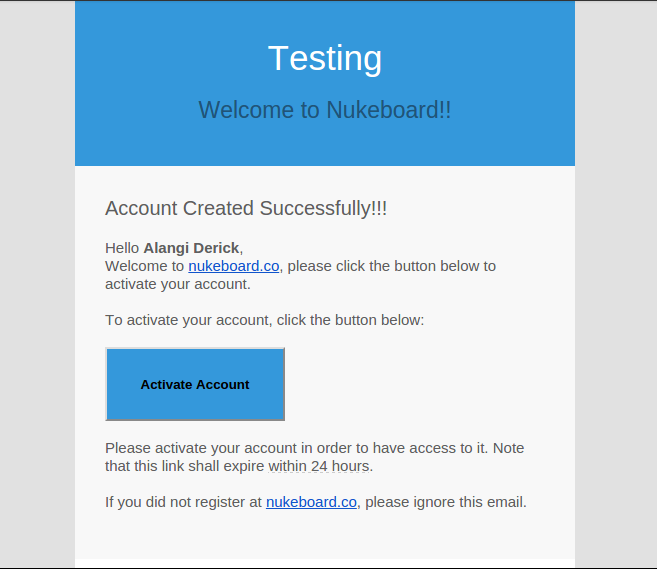
\includegraphics[width=13cm,scale=1.5]{Figures/HTMLEmail}
\decoRule
\caption[HTML Email]{HTML email for account activation}
\label{fig:HTMLEmail}
\end{figure} 

\subsection{Testing/Quality Assurance(QA) on Nukeboard(nukeboard.co)}

This is a very important key aspect in software engineering. It is to make sure that all aspects of a software is working well and as expected. Basically, its a process carried out to know the performance of a system, what to improve, change and more... \\

Formally, \textbf{\textit{Quality Assurance}} is the maintenance of a desired level of quality in a service or product, especially by means of attention to every stage of the process of delivery or production. \\

This task was assigned to me during my internship period and even though I did not finish testing the whole software, I tested about 80\% of the whole software and at the end of the testing, I had a total of 53 test cases spanning across various functionalities of the software. I was instructed to create and online spreed sheet(Google Spread Sheet) and give it access to all members in the nukeboard development team so that if there is a test carried out of my own tests, it can be added and when maintenance is being done, all will be included and worked upon. The sheet was created and the link can be found at [x] which holds information about all the test cases.

\subsubsection{Statistics of the QA}

Below is a table showing the number of test carried out, the onces that failed and those that passed. Also those that need improvement also need to be improved. \\

\begin{tabular}{ |p{3cm}|p{3cm}|p{3cm}|p{3cm}|  }
 \hline
 \multicolumn{4}{|c|}{Quality Assurance Statistics} \\
 \hline
 Number of Test Cases & Tests passed & Tests failed & Test that need improvement\\
 \hline
 53  & 37 & 13 & 3\\
 \hline
\end{tabular}

\subsubsection{Explanation of text results}

\textbf{Passed }means that the test was carried out and the expected output was equal to the users output or the output of the existing system. \\

\textbf{Failed }are the various test cases whose output was not as expected meaning there is something not working in the software as it is suppose to work. Cases like this needs to be looked into and fixed.

\textbf{Improvement } is a test that actually passed and did work as expected but there is a way of improving this functionality to make it look better to the user at the moment. Cases like this can be look into but not urgently.

At the end of this testing, the statistic gathered will be showed in percentage pass and failed in the results section of this report. Including other results, everything shall be revealed in the discussion and results section of the report.

